\documentclass[11pt,letterpaper]{article}
\usepackage[T1]{fontenc}
\usepackage{lmodern}
\usepackage[margin=0.8in,headheight=15pt]{geometry}
\usepackage{amsmath,amssymb,booktabs,array,xcolor,tikz,fancyhdr}
\usepackage[hidelinks]{hyperref}
\usetikzlibrary{arrows.meta}
\definecolor{ink}{HTML}{16384B}
\definecolor{accent}{HTML}{087E8B}
\definecolor{pale}{HTML}{EFF6F8}
\pagestyle{fancy}\fancyhf{}
\fancyhead[L]{\small\textcolor{ink}{Electromagnetism: laws and experiments}}
\fancyhead[R]{\small Learning note}
\fancyfoot[L]{\footnotesize Updated 6 October 2026}
\fancyfoot[R]{\thepage}
\setlength{\parindent}{0pt}\setlength{\parskip}{5pt}
\setlength{\emergencystretch}{2em}
\newcolumntype{P}[1]{>{\raggedright\arraybackslash}p{#1}}
\newcommand{\vect}[1]{\boldsymbol{#1}}
\newcommand{\dd}{\,\mathrm d}
\newcommand{\idea}[1]{\par\smallskip\noindent\colorbox{pale}{\parbox{\dimexpr\linewidth-2\fboxsep\relax}{#1}}\par\smallskip}
\hypersetup{pdftitle={Electromagnetism: Laws, Experiments and Their Relationships},pdfauthor={Learning-Note}}
\begin{document}
\begin{center}
{\LARGE\bfseries\color{ink} Electromagnetism Foundations}\\[6pt]
{\large Laws, experiments, and their relationships}\\[6pt]
{\small A historical timeline with physical and mathematical explanations\\6 October 2026}
\end{center}

\section*{How to read this note}
This is the second note in this topic. The companion \texttt{fields-and-vector-calculus.tex} explains field measurement, magnetic moments and spin, and flux, divergence, and curl. This note organizes the laws already discussed, with particular attention to the experimental meaning of Faraday's law and the distinction between EMF and electric field. Wave propagation, transmission-line reflection, and analysis of the AN720 remain future lessons.

\begin{tabular}{P{0.20\linewidth}P{0.73\linewidth}}
\toprule
Statement & What establishes it?\\\midrule
Definition & Specifies a quantity and an operational way to determine it.\\
Mathematical theorem & A proof from definitions and assumptions about the functions and geometry.\\
Physical law & Experimental evidence. Mathematics can derive consequences once the law is accepted.\\\bottomrule
\end{tabular}

\section*{Historical map}
\begin{tabular}{P{0.20\linewidth}P{0.73\linewidth}}
\toprule
Period & Development and its role\\\midrule
1785 & Coulomb: quantitative force between stationary charges.\\
1820 onward & \O rsted, Biot--Savart, and Amp\`ere: magnetic effects and interactions of steady currents.\\
19th century & Overlapping mathematical development: potential theory, surface flux, and integral theorems; the electrostatic Gauss relationship.\\
1831 & Faraday: electromagnetic induction, including electrically isolated stationary coils.\\
1834 & Lenz: the direction of induced current.\\
1850s & Thomson--Stokes circulation theorem; printed in an 1854 examination.\\
1860s & Maxwell: completion of the time-dependent field equations.\\
Later 19th century & Modern combined force-law formulation associated with Lorentz, with earlier contributions.\\\bottomrule
\end{tabular}

Dates refer to developments, not first appearances of the exact modern equations used here. Mathematics and electromagnetism developed partly alongside one another; there is no universal sequence in which all vector-calculus definitions were completed before electromagnetic theory. Historical order also differs from logical dependence: a later theory can derive an earlier result.

\newpage
\section{1785: Coulomb's law and the electric-field definition}
\subsection*{Observation before formula}
Coulomb used a calibrated torsion balance. Electric force twisted a suspended assembly; its twist provided a measure of force. Varying separation supported an inverse-square dependence. A force measurement is the experimental input, not a conclusion drawn from an assumed electric-field formula.\cite{coulomb}

For stationary point charges in vacuum, the modern law is
\begin{equation}
\vect F_E=\frac{Qq}{4\pi\varepsilon_0r^2}\hat{\vect r}.
\end{equation}
$Q$ is the source charge, $q$ the probe charge, $r$ their separation, and $\hat{\vect r}$ points from source to probe. Signed charges determine attraction or repulsion. $\varepsilon_0$ is the vacuum electric constant. The charge dependence and inverse-square dependence are physical claims established through measurements.

\subsection*{Definition and derived result}
The electric field is the external electric force per signed, sufficiently small test charge in a specified frame:
\begin{equation}
\vect E=\lim_{q\to0}\frac{\vect F_E}{q}.
\end{equation}
The limit expresses negligible disturbance of the sources. Its direction is the electric-force direction for a positive probe; units are $\mathrm{N/C}=\mathrm{V/m}$.

Substituting Coulomb's law gives
\begin{equation}
\vect E=\frac{Q}{4\pi\varepsilon_0r^2}\hat{\vect r}.
\end{equation}
\idea{\textbf{Logical relationship:} measured Coulomb force law + electric-field definition $\longrightarrow$ point-charge field formula. Defining $\vect E$ does not prove how a source produces it.}

\subsection*{Physical interpretation}
The field separates the environment's effect from the particular probe. If the probe charge doubles while the source remains undisturbed, its electric force doubles; the inferred field stays the same. A negative probe feels force opposite to the field.

Coulomb's equation applies to electrostatics. It must not be used as an instantaneous source formula for arbitrary changing fields. General time-dependent electromagnetism requires the full field equations.

\newpage
\section{1820 onward: magnetic effects of steady currents}
\subsection*{What the demonstrations establish}
\O rsted observed compass deflection near a battery-connected wire. Amp\`ere investigated attraction and repulsion between current-carrying conductors. These observations established a physical connection between electric currents and magnetism. A single compass deflection does not establish a complete quantitative field law.\cite{amperehistory}

\subsection*{Biot--Savart: quantitative source law}
For a steady filamentary current in vacuum,
\begin{equation}
\vect B(\vect r)=\frac{\mu_0}{4\pi}
\int_{\text{circuit}}\frac{I\dd\vect\ell'\times\hat{\vect R}}{R^2}.
\end{equation}
$\mu_0$ is the vacuum magnetic constant; $\dd\vect\ell'$ follows conventional current in the source wire. $\vect R$ points from the source element to the observation point. The cross product specifies the contribution's direction. The integral adds contributions from the complete current distribution; a current element is a mathematical contribution, not an independently isolated steady-current source.\cite{biotsavart}

The source law is empirically grounded. Evaluating its integral for a specified geometry is a mathematical derivation. For an ideal infinitely long straight wire, with $z$ along the wire and $r$ the perpendicular distance,
\begin{equation}
B=\frac{\mu_0I}{4\pi}\int_{-\infty}^{\infty}
\frac{r\dd z}{(r^2+z^2)^{3/2}}
=\frac{\mu_0I}{2\pi r}.
\end{equation}
The field runs around the wire, with direction set by the current. This is a derived geometry-specific result.

\subsection*{Amp\`ere's circuital law}
The modern magnetostatic circulation law is
\begin{equation}
\oint_C\vect B\cdot\dd\vect\ell=\mu_0I_{\text{through }S},
\qquad C=\partial S.
\end{equation}
The left side accumulates the tangential magnetic field around a chosen path. The right side is the signed current crossing a spanning surface, with matching orientation. The path is mathematical and need not be a wire.\cite{ampere}

For a circle around the straight wire, $\vect B$ is tangent and has constant magnitude, so
\[
\oint_C\vect B\cdot\dd\vect\ell=B(2\pi r)=\mu_0I.
\]
This checks agreement for one geometry; it is not a proof for every current distribution. Biot--Savart and the magnetostatic field equations describe the same physics with appropriate boundary conditions. The steady-current restriction matters: a time-dependent extension appears later.

\newpage
\section{The mathematical branch: flux, divergence, and Gauss's law}
\subsection*{Flux is a definition}
For an oriented surface $S$,
\begin{equation}
\Phi_F=\int_S\vect F\cdot\hat{\vect n}\dd A.
\end{equation}
$\dd A$ is a scalar area patch; $\hat{\vect n}$ its unit normal. The dot product selects the component crossing the patch. Flux adds those crossing contributions; it need not represent material flowing.

\subsection*{Deriving the electrostatic Gauss relationship}
Surround a charge $Q$ with a sphere. Its Coulomb field is normal to the sphere and constant in magnitude there:
\[
\oint_S\vect E\cdot\hat{\vect n}\dd A
=E(r)4\pi r^2
=\frac{Q}{4\pi\varepsilon_0r^2}4\pi r^2
=\frac{Q}{\varepsilon_0}.
\]
The inverse-square field decrease compensates exactly for the sphere's increasing area. For a general surface, a patch subtends signed solid angle $\dd\Omega=(\hat{\vect r}\cdot\hat{\vect n})\dd A/r^2$ at the charge. Its electric flux is $Q\dd\Omega/(4\pi\varepsilon_0)$. A closed surface has total signed solid angle $4\pi$ for an inside charge and zero for an outside charge. Adding charge contributions by superposition gives
\begin{equation}
\boxed{\oint_{\partial V}\vect E\cdot\hat{\vect n}\dd A
=\frac{Q_{\text{inside}}}{\varepsilon_0}.}
\end{equation}
This derives the electrostatic flux law from Coulomb plus superposition. Its validity for general changing fields is a broader physical statement.\cite{gauss}

\subsection*{The divergence theorem is mathematics}
\begin{equation}
\oint_{\partial V}\vect F\cdot\hat{\vect n}\dd A
=\int_V\nabla\cdot\vect F\dd V.
\end{equation}
For a tiny box, differences on opposite faces give net outward flux approximately equal to
\[
\left(\frac{\partial F_x}{\partial x}+\frac{\partial F_y}{\partial y}
+\frac{\partial F_z}{\partial z}\right)\Delta V.
\]
As boxes are joined, contributions through shared internal faces cancel. Taking the limit leaves only the outside boundary. This is the proof structure for regular fields and regions.

Combining the theorem with electric Gauss's law gives $\int_V(\nabla\cdot\vect E-\rho/\varepsilon_0)\dd V=0$ for arbitrary volumes, hence
\begin{equation}
\boxed{\nabla\cdot\vect E=\rho/\varepsilon_0.}
\end{equation}
$\rho$ is charge density. The theorem converts total flux to local divergence; the physical law relates the electric field to charge.

\newpage
\section{1831: Faraday's experiment and the meaning of EMF}
\subsection*{Apparatus and observations}
Faraday placed two electrically insulated windings on an iron ring. One connected to a battery; the other to a galvanometer. There was no conducting connection between the windings. His successful induction experiment occurred on 29 August 1831.\cite{ring}

\begin{tabular}{P{0.43\linewidth}P{0.50\linewidth}}
\toprule
Source circuit & Receiving circuit\\\midrule
Battery connected & Brief current in one direction.\\
Battery left connected; conditions settle & Current returns to zero.\\
Battery disconnected & Brief current in the opposite direction.\\\bottomrule
\end{tabular}

The source current establishes a magnetic field. Connection and disconnection change it; a settled field does not sustain induced current. These observations establish induction qualitatively. They do not alone establish every factor in the quantitative formula.\cite{faraday}

\subsection*{EMF is a circuit driving quantity}
EMF means \emph{electromotive force}, but is not a mechanical force. It measures driving action per unit charge around a circuit and has unit volt: $1\,\mathrm V=1\,\mathrm{J/C}$. For stationary-loop electromagnetic induction,
\begin{equation}
\boxed{\mathcal E=\oint_C\vect E\cdot\dd\vect\ell.}
\end{equation}
At each point, $\vect E$ is the actual field (force direction for a positive test charge). $\dd\vect\ell$ is tangent to the path in our chosen traversal direction. It is a reference direction, not an assumption about electron motion.
\[
\vect E\cdot\dd\vect\ell=|\vect E|\dd\ell\cos\theta.
\]
Aligned directions give positive contributions, opposite directions negative, and perpendicular directions zero. The integral accumulates the tangential driving action at the same instant. In a changing field, it is not automatically the work along a charge's finite-time journey.\cite{induction}

\begin{center}
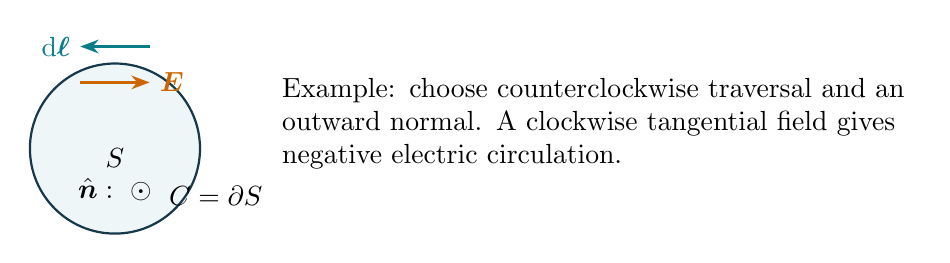
\begin{tikzpicture}[>=Stealth,scale=0.8]
\fill[pale] (0,0) circle (1.35);
\draw[thick,ink] (0,0) circle (1.35);
\draw[->,thick,accent] (0.55,1.62)--(-0.55,1.62) node[left] {$\dd\vect\ell$};
\draw[->,thick,orange!80!black] (-0.55,1.05)--(0.55,1.05) node[right] {$\vect E$};
\node at (0,-0.15) {$S$};
\node at (0,-0.65) {$\hat{\vect n}:\ \odot$};
\node at (1.6,-0.75) {$C=\partial S$};
\node[align=left,anchor=west,text width=8cm] at (2.5,0.4) {Example: choose counterclockwise traversal and an outward normal. A clockwise tangential field gives negative electric circulation.};
\end{tikzpicture}
\end{center}
EMF quantifies the field's driving action. It is not a separate object created by the field. Current is the circuit's response; resistance and inductance affect that response.

\newpage
\section{Faraday's quantitative law: what must be measured independently}
For a stationary loop bounding a fixed surface,
\begin{equation}
\boxed{\mathcal E=-\frac{\mathrm d\Phi_B}{\mathrm dt},\qquad
\Phi_B=\int_S\vect B\cdot\hat{\vect n}\dd A.}
\end{equation}
Thus
\begin{equation}
\boxed{\oint_C\vect E\cdot\dd\vect\ell
=-\frac{\mathrm d}{\mathrm dt}\int_S\vect B\cdot\hat{\vect n}\dd A.}
\end{equation}
\textbf{Left:} electric driving action around the one-dimensional boundary $C$. \textbf{Right:} negative magnetic-flux change rate through the two-dimensional spanning surface $S$. The normal and traversal follow the right-hand rule. They are different geometric objects, related by $C=\partial S$.

\subsection*{Why the equality is a physical law}
Neither quantity's definition forces them to be equal. A modern test can determine both independently:
\begin{enumerate}
\item Measure the receiving loop's resistance separately and its current during induction. For slow changes with negligible inductive effects, infer $\mathcal E\approx RI$ from the independently established resistive response.
\item Measure magnetic field by magnetic-force effects, rather than calculating it from the induction formula. Measure the surface geometry. For uniform perpendicular field and fixed area, the flux definition gives $\Phi_B=BA$ and its change rate is $A\,\mathrm dB/\mathrm dt$.
\item Compare $RI$ with $-A\,\mathrm dB/\mathrm dt$ while changing area, field-change rate, and direction. Changing resistance tests whether the driving quantity stays the same while current changes.
\end{enumerate}
This describes a way to test the law, not a claim that Faraday's original ring experiment performed every measurement. Repeated experiments support the general relationship.\cite{faraday}

The receiving current creates its own magnetic field. In the simple comparison it is made negligible, or its contribution must be included. The exact field equation uses the total $\vect B$; rapid transients require accounting for inductance rather than assuming $\mathcal E=RI$ for the imposed field alone.

\subsection*{Concrete prediction}
A fixed loop with $A=0.01\,\mathrm{m^2}$ experiences a perpendicular field increase $\Delta B=0.1\,\mathrm T$. Then $\Delta\Phi_B=0.001\,\mathrm{Wb}$. The predicted average EMF magnitude is $0.001\,\mathrm V$ if the change takes $1\,\mathrm s$, and $0.01\,\mathrm V$ if it takes $0.1\,\mathrm s$. The same endpoints give different driving action because the change rate differs. These are illustrative predictions, not invented historical measurements.

\idea{\textbf{Physical meaning:} changing linked magnetic flux is associated with an electric field having net circulation. That field acts on charges; EMF measures its circuit driving action. The field can exist without a wire. Classical electromagnetism takes this relationship as a basic physical law, not a consequence of the definitions.\cite{inducedE}}

\newpage
\section{1834: Lenz's law and orientation}
Lenz formulated the direction rule for induced currents in 1834.\cite{lenz}

In an ordinary passive conducting loop, the induced current's magnetic effect opposes the change in flux responsible for induction. It does not always oppose the existing magnetic field.

\subsection*{Reading the minus sign}
For a symmetric circular loop, choose $\hat{\vect n}$ out of the page. The matching positive traversal is counterclockwise:
\begin{itemize}
\item Increasing outward flux gives $\mathrm d\Phi_B/\mathrm dt>0$.
\item Faraday's law gives $\mathcal E<0$ relative to the chosen traversal.
\item The tangential induced electric driving action is clockwise.
\item Conventional induced current is clockwise and contributes an inward magnetic field.
\end{itemize}
If outward flux decreases, the induced current contributes an outward field, opposing the decrease. Reversing the reference normal also reverses the traversal and both signed sides of Faraday's equation; it does not change the physical phenomenon.

\subsection*{What energy conservation does and does not establish}
For a passive loop, opposition is consistent with the work needed to impose the magnetic change. Energy comes from the source maintaining that change; it is dissipated or stored in the receiving system. Energy conservation constrains the interpretation but does not, by itself, determine every factor in Faraday's quantitative magnitude law.

\subsection*{Electric field versus magnetic force}
The induced circuit driving action is electric. The magnetic force on a point charge, $q\vect v\times\vect B$, is perpendicular to its velocity and does no instantaneous work on it. The induced electric field can supply energy to moving charges. A change in magnetic flux and an electric driving action are related aspects of the induction phenomenon, not two independent EMFs that should be added.

For a fixed loop with zero flux-change rate, the net induced EMF is zero. That statement does not imply that all electric fields everywhere vanish, or that current in an inductive circuit disappears instantly.

\newpage
\section{1850s: Stokes' theorem and the local form of induction}
The theorem communicated by William Thomson to Stokes appeared in print in an 1854 examination. It is mathematical and applies to vector fields in fluid mechanics and other subjects as well as electromagnetism.\cite{tong}
\begin{equation}
\boxed{\oint_C\vect F\cdot\dd\vect\ell
=\int_S(\nabla\times\vect F)\cdot\hat{\vect n}\dd A.}
\end{equation}
It says that total boundary circulation equals the sum of local normal curl across the spanning surface. Curl measures infinitesimal circulation per area, rather than simply whether drawn field lines look curved.

\subsection*{Proof structure}
For a small rectangle in the $xy$ plane traversed counterclockwise, the two horizontal edges contribute approximately $-(\partial F_x/\partial y)\Delta x\Delta y$, while the vertical edges contribute $(\partial F_y/\partial x)\Delta x\Delta y$. Their sum is
\[
\oint_{\text{rectangle}}\vect F\cdot\dd\vect\ell
\approx\left(\frac{\partial F_y}{\partial x}-\frac{\partial F_x}{\partial y}\right)\Delta A.
\]
The bracket is the normal component of curl. Joining patches cancels circulation contributions along shared internal edges. Taking the limit gives the theorem; a curved surface is handled by oriented local patches with suitable smoothness. This establishes a mathematical relation, not a law about magnetic change.

\subsection*{Apply the theorem after accepting Faraday's physical law}
For a fixed $S$, Stokes' theorem and differentiation under the integral give
\begin{align}
\int_S(\nabla\times\vect E)\cdot\hat{\vect n}\dd A
&=-\int_S\frac{\partial\vect B}{\partial t}\cdot\hat{\vect n}\dd A,\\
\int_S\left(\nabla\times\vect E+\frac{\partial\vect B}{\partial t}\right)
\cdot\hat{\vect n}\dd A&=0.
\end{align}
Because this holds for arbitrary sufficiently small surfaces and orientations in regular regions,
\begin{equation}
\boxed{\nabla\times\vect E=-\frac{\partial\vect B}{\partial t}.}
\end{equation}
This is the local form of the same Faraday law. Stokes proves equivalence of forms; experiments support their physical content.

Similarly, writing $I_{\text{through }S}=\int_S\vect J\cdot\hat{\vect n}\dd A$ and applying Stokes to steady-current Amp\`ere's law gives
\begin{equation}
\boxed{\nabla\times\vect B=\mu_0\vect J.}
\end{equation}
$\vect J$ is current density, a directed charge flow per unit area.

\newpage
\section{The 1860s: Maxwell and time-dependent fields}
\subsection*{Why the steady-current equation needs an extension}
Charge conservation says that net outward charge flow decreases the charge stored in a volume:
\[
\frac{\mathrm d}{\mathrm dt}\int_V\rho\dd V
=-\oint_{\partial V}\vect J\cdot\hat{\vect n}\dd A.
\]
The divergence theorem converts this balance to
\begin{equation}
\nabla\cdot\vect J=-\frac{\partial\rho}{\partial t}.
\end{equation}
But the old Amp\`ere equation implies $\nabla\cdot\vect J=0$, since the divergence of a sufficiently smooth curl is mathematically zero. That is compatible with steady conditions, but not arbitrary charge accumulation.

\subsection*{The additional electric-field term}
Maxwell's extension in modern microscopic vacuum notation is
\begin{equation}
\boxed{\nabla\times\vect B=\mu_0\vect J
+\mu_0\varepsilon_0\frac{\partial\vect E}{\partial t}.}
\end{equation}
Electric Gauss's law gives
\[
\nabla\cdot\left(\varepsilon_0\frac{\partial\vect E}{\partial t}\right)
=\frac{\partial\rho}{\partial t}.
\]
Its divergence cancels the current contribution required by conservation. This is a modern consistency argument motivating the extension, not a unique proof that nature must obey it or a complete reconstruction of Maxwell's historical reasoning. Experiments support the completed theory.\cite{maxwell}

Its integral form follows through Stokes:
\begin{equation}
\oint_C\vect B\cdot\dd\vect\ell
=\mu_0\int_S\vect J\cdot\hat{\vect n}\dd A
+\mu_0\varepsilon_0\frac{\mathrm d}{\mathrm dt}\int_S\vect E\cdot\hat{\vect n}\dd A.
\end{equation}
It relates magnetic circulation to current crossing the surface and changing electric flux. The added term is often called the displacement-current term; it does not require material charge carriers crossing every part of the surface.

\subsection*{The other magnetic equation}
Standard classical electromagnetism has no magnetic-monopole sources:
\begin{equation}
\boxed{\nabla\cdot\vect B=0,\qquad
\oint_{\partial V}\vect B\cdot\hat{\vect n}\dd A=0.}
\end{equation}
The divergence theorem relates these forms. The zero net flux is a physical statement about magnetic fields, not a consequence of the definition of divergence. This note records the equation as part of the law map; it does not begin a separate lesson on monopoles or wave propagation.

\newpage
\section{Modern force law and the force on a wire}
The combined expression associated with Lorentz is
\begin{equation}
\boxed{\vect F=q(\vect E+\vect v\times\vect B).}
\end{equation}
Its history includes contributions before the later nineteenth-century formulation associated with Lorentz; assigning the entire discovery to one author and year is misleading.\cite{forcehistory}

$q\vect E$ is electric force, including on a stationary probe. $q\vect v\times\vect B$ is magnetic force. Its magnitude is $F_B=|q|vB\sin\theta$, and therefore $B=F_B/(|q|v)$ for perpendicular motion. Measurements with several velocity directions determine the vector field; one velocity direction misses the component parallel to it. The force relationship is experimentally grounded and supplies an operational measurement of $\vect B$.

\subsection*{Deriving the straight-wire force}
Consider carriers of signed charge $q$, number density $n$, drift velocity $\vect v_d$, and wire cross-sectional area $a$. A straight segment of length $L$ contains $naL$ carriers. In a uniform external field, summing their magnetic forces gives
\begin{align}
\vect F&=naLq\vect v_d\times\vect B,\\
\vect J&=nq\vect v_d,\\
\vect F&=aL\vect J\times\vect B
=I\vect\ell\times\vect B.
\end{align}
$\vect\ell$ points along conventional current and has length $L$. This result assumes the wire's carriers transfer their force to the material in the usual conductor description. Contributions from multiple carrier species can be added.

\idea{\textbf{Two different jobs:} Maxwell's equations govern fields and their relation to sources and changes. The force law governs how charges respond to those fields. Knowing a field does not specify particle motion until its force and the equation of motion are supplied.}

\section*{Where the present lesson stops}
The next lesson should develop one Maxwell law or its physical interpretation at a time, after understanding is confirmed. The mathematical prediction of propagating waves, conductor boundary behavior, guided transmission-line fields, and reflection at a short remain later subjects. The antenna photograph alone does not establish its complete electromagnetic structure.

\newpage
\section*{Relationship map}
\begin{tabular}{P{0.29\linewidth}P{0.32\linewidth}P{0.30\linewidth}}
\toprule
Relationship & Physical input & Mathematical connection\\\midrule
Coulomb force to point-charge $\vect E$ & Coulomb force law & Definition $\vect E=\vect F_E/q$.\\
Coulomb to electrostatic Gauss flux & Coulomb and superposition & Geometry and integration.\\
Gauss flux to divergence & Electric Gauss law & Divergence theorem and arbitrary volumes.\\
Magnetic-flux change to electric circulation & Faraday induction law & EMF and flux definitions identify the measured quantities.\\
Faraday circulation to curl & Same Faraday law & Stokes, fixed surface, and arbitrary local patches.\\
Steady Amp\`ere circulation to curl & Steady-current magnetic law & Stokes and current-density definition.\\
Steady Amp\`ere to Maxwell extension & Added time-dependent physical relationship & Charge-conservation consistency motivates the new term.\\
Charge force to wire force & Magnetic-force law & Sum carrier forces; use current's definition.\\\bottomrule
\end{tabular}

\section*{Scope and compilation}
All force and source formulas above use SI units and external probe fields where appropriate. The displayed $\vect E,\vect B$ Maxwell equations use total microscopic charge and current; a macroscopic material formulation requires care with polarization, magnetization, $\vect D$, and $\vect H$. Integral laws handle ideal source singularities better than ordinary pointwise derivatives.

This source is self-contained. Upload \texttt{laws-experiments-and-timeline.tex} to Overleaf, select it as the main document, and use pdfLaTeX. On a standard local TeX installation, compile twice:
\begin{verbatim}
pdflatex -interaction=nonstopmode -halt-on-error \
  laws-experiments-and-timeline.tex
\end{verbatim}
The diagram and bibliography are embedded. No external images, BibTeX, shell escape, or machine-specific paths are required.

\newpage
The sources below support historical attribution, physical interpretation, and the law map. Proof sketches and numerical illustrations are explanatory reconstructions, not claimed original laboratory records.
\begin{thebibliography}{99}\small
\bibitem{coulomb} American Physical Society, \emph{June 1785: Coulomb Measures the Electric Force}. \url{https://www.aps.org/apsnews/2016/06/coulomb-measures-electric-force}.
\bibitem{amperehistory} Amp\`ere historical archive, \emph{Amp\`ere lays the foundations of electrodynamics}. \url{https://ampere-archives.fr/histoire-electricite/parcours-historique/lois-courants/ampere-electrodynamique/eng}.
\bibitem{biotsavart} OpenStax, University Physics Volume 2, \S12.1, \emph{The Biot--Savart Law}. \url{https://openstax.org/books/university-physics-volume-2/pages/12-1-the-biot-savart-law}.
\bibitem{ampere} OpenStax, \S12.5, \emph{Amp\`ere's Law}. \url{https://openstax.org/books/university-physics-volume-2/pages/12-5-amperes-law}.
\bibitem{gauss} OpenStax, \S6.2, \emph{Explaining Gauss's Law}. \url{https://openstax.org/books/university-physics-volume-2/pages/6-2-explaining-gausss-law}.
\bibitem{ring} Royal Institution, \emph{Michael Faraday's ring-coil apparatus}. \url{https://www.rigb.org/explore-science/explore/collection/michael-faradays-ring-coil-apparatus}.
\bibitem{faraday} OpenStax, \S13.1, \emph{Faraday's Law}. \url{https://openstax.org/books/university-physics-volume-2/pages/13-1-faradays-law}.
\bibitem{induction} Feynman Lectures, Volume II, Chapter 17, \emph{The Laws of Induction}. \url{https://www.feynmanlectures.caltech.edu/II_17.html}.
\bibitem{inducedE} OpenStax, \S13.4, \emph{Induced Electric Fields}. \url{https://openstax.org/books/university-physics-volume-2/pages/13-4-induced-electric-fields}.
\bibitem{lenz} E. Lenz (1834), \emph{Ueber die Bestimmung der Richtung der durch elektrodynamische Vertheilung erregten galvanischen Str\"ome}. \url{https://doi.org/10.1002/andp.18341073103}.
\bibitem{tong} David Tong, \emph{Vector Calculus}, Chapter 4, integral theorems and Stokes history. \url{https://www.damtp.cam.ac.uk/user/tong/vc/vc.pdf}.
\bibitem{maxwell} Feynman Lectures, Volume II, Chapter 18, \emph{The Maxwell Equations}. \url{https://www.feynmanlectures.caltech.edu/II_18.html}.
\bibitem{forcehistory} G. Giuliani, \emph{Maxwell's derivation of the Lorentz force from Faraday's law} (2019). \url{https://arxiv.org/abs/1911.04605}.
\end{thebibliography}
\end{document}
